% !TEX program = xelatex
\documentclass[12pt,a4paper]{article}
\usepackage[margin=2.2cm]{geometry}
\usepackage{graphicx}
\usepackage{booktabs}
\usepackage{longtable}
\usepackage{array}
\usepackage{amsmath}
\usepackage{float}
\usepackage{caption}
\usepackage{xepersian}
\settextfont{Amiri}
\setdigitfont{Amiri}
\setlatintextfont{DejaVu Serif}
\setlatinmonofont{DejaVu Sans Mono}
\linespread{1.25}
\graphicspath{{plots/}}
\newcommand{\en}[1]{\lr{#1}}
\newcommand{\Mbps}{\en{Mbps}}

\title{\textbf{پروژهٔ سوم درس ارتباطات داده}\\[4pt]
کنترل جریان و انتقال قابل‌اعتماد در \en{ns-3}}
\author{نام دانشجو: \rule{5cm}{0.4pt}\\ شماره دانشجویی: \rule{4cm}{0.4pt}}
\date{آبان ۱۴۰۵}

\begin{document}
\maketitle
\vspace{-0.4cm}
\begin{center}
\textbf{دو گره متصل با یک پیوند نقطه‌به‌نقطه؛ بدون استفاده از \en{Wi-Fi}}\\
\vspace{4pt}
\rule{0.9\textwidth}{0.4pt}
\end{center}

\section{چکیده}
در این پروژه سه سازوکار \en{ARQ} شامل توقف‌و‌انتظار، بازگشت به عقب \en{(Go-Back-N)} و تکرار انتخابی \en{(Selective Repeat)} بررسی شده‌اند. پیاده‌سازی اصلی در فایل \en{scratch/arq-hw3.cc} برای محیط \en{ns-3.46} نوشته شده است. پروتکل‌های \en{DATA/ACK} در لایه‌ای بالاتر از دو دستگاه \en{PointToPointNetDevice} و با سرآیند اختصاصی پیاده‌سازی می‌شوند؛ بنابراین قابلیت اطمینان به خود دستگاه نقطه‌به‌نقطه واگذار نشده است. خروجی برنامه شامل توان‌گذردهی مفید، میانگین تأخیر تحویل، تعداد بازفرست‌ها، تعداد انقضای زمان‌سنج و شاخص‌های بافر گیرنده است.

\textbf{ملاحظهٔ مهم دربارهٔ داده‌های این نسخه:} محیط اجرایی فعلی به \en{Docker} یا کتابخانه‌های \en{ns-3} دسترسی ندارد؛ در نتیجه فایل‌های \en{CSV} و نمودارهای ضمیمه برای پیش‌نمایش، از مدل مرجع رویدادگسستهٔ همراه پروژه تولید شده‌اند و نباید به‌عنوان خروجی اجرای واقعی \en{ns-3} معرفی شوند. کد \en{ns-3} آمادهٔ اجرا در تصویر Docker درس است و پس از اجرای آن، فایل \en{results/ns3\_results.csv} و نمودارها باید با داده‌های واقعی جایگزین شوند. این محدودیت در README نیز توضیح داده شده است.

\section{ساختار آزمایش و فرض‌ها}
در همهٔ آزمایش‌ها دقیقاً دو گره با یک پیوند نقطه‌به‌نقطهٔ تمام‌دوطرفه به هم متصل‌اند. از \en{Wi-Fi}، پشتهٔ \en{IP}، ‏\en{UDP} و ‏\en{TCP} استفاده نشده است. پیام‌های داده و تأیید دریافت، سرآیند اختصاصی پنج‌بایتی دارند. اندازهٔ محمولهٔ داده \en{1000 byte} است؛ سربار سرآیند پروتکل و قاب‌بندی نقطه‌به‌نقطه در نرخ ارسال لینک لحاظ می‌شود، اما در محاسبهٔ توان‌گذردهی فقط بایت‌های محمولهٔ یکتای تحویل‌شده شمرده می‌شوند.

\begin{table}[H]
\centering
\caption{پارامترهای پایهٔ آزمایش}
\begin{tabular}{>{\raggedleft\arraybackslash}p{6cm}p{6cm}}
\toprule
پارامتر & مقدار \\
\midrule
تعداد گره‌ها و نوع اتصال & دو گره، یک پیوند \en{Point-to-Point} \\
نرخ لینک & \en{10 Mbps} \\
تأخیر انتشار یک‌طرفهٔ پایه & \en{5 ms} \\
اندازهٔ محموله & \en{1000 byte} \\
مدت شبیه‌سازی و بازهٔ مشاهده & \en{30 s} \\
ظرفیت پیش‌فرض بافر خارج از ترتیب & \en{20} بسته \\
احتمال اتلاف پایه & \en{0} \\
زمان‌سنج بازفرست & \en{100 ms} \\
بذر تصادفی & \en{12345} \\
ترافیک فرستنده & اشباع؛ ارسال بستهٔ بعدی با آزاد شدن پنجره \\
\bottomrule
\end{tabular}
\end{table}

در آزمایش‌های اتلاف، احتمال حذف هر قاب \en{DATA} و هر قاب \en{ACK} مستقل از دیگری و برابر \en{$p$} است. حذف \en{DATA} در سمت گیرنده و حذف \en{ACK} در سمت فرستنده اعمال می‌شود. برای تکرارپذیری، بذر تصادفی ثابت است و جریان‌های تصادفی جداگانه برای \en{DATA} و \en{ACK} در نظر گرفته شده‌اند.

\section{معیارهای اندازه‌گیری}
اگر \en{$N_u$} تعداد محموله‌های یکتای تحویل‌شده، \en{$L$} اندازهٔ محموله برحسب بایت و \en{$T_{obs}$} زمان مشاهده باشد، توان‌گذردهی مفید از رابطهٔ زیر به دست می‌آید:
\[
G=\frac{8 L N_u}{T_{obs}}.
\]
میانگین تأخیر، فاصلهٔ زمانی از نخستین فراخوانی \en{NetDevice::Send} برای هر بسته تا تحویل مرتب آن در گیرنده است؛ بنابراین اگر دستگاه در صف ارسال داشته باشد، انتظار در صف دستگاه نیز در این مقدار منظور می‌شود:
\[
\bar D=\frac{1}{N_u}\sum_{i=1}^{N_u}(t_{i,delivery}-t_{i,first}).
\]
نسبت بازفرست نیز برابر تعداد ارسال‌های مجدد تقسیم بر تعداد بسته‌های یکتای تحویل‌شده است. هر محموله فقط یک بار در توان‌گذردهی و میانگین تأخیر شمرده می‌شود؛ نسخه‌های تکراری در گیرنده دوباره تحویل لایهٔ بالاتر داده نمی‌شوند.

\section{مسئلهٔ اول: توقف‌و‌انتظار}
\subsection{اثر تأخیر انتشار}
در این آزمایش احتمال اتلاف صفر و تأخیر یک‌طرفه به‌ترتیب \en{1}، ‏\en{5} و ‏\en{20 ms} است. نمودار شکل~\ref{fig:sw-delay} افت توان‌گذردهی با افزایش زمان رفت‌وبرگشت را نشان می‌دهد.

\begin{figure}[H]
\centering
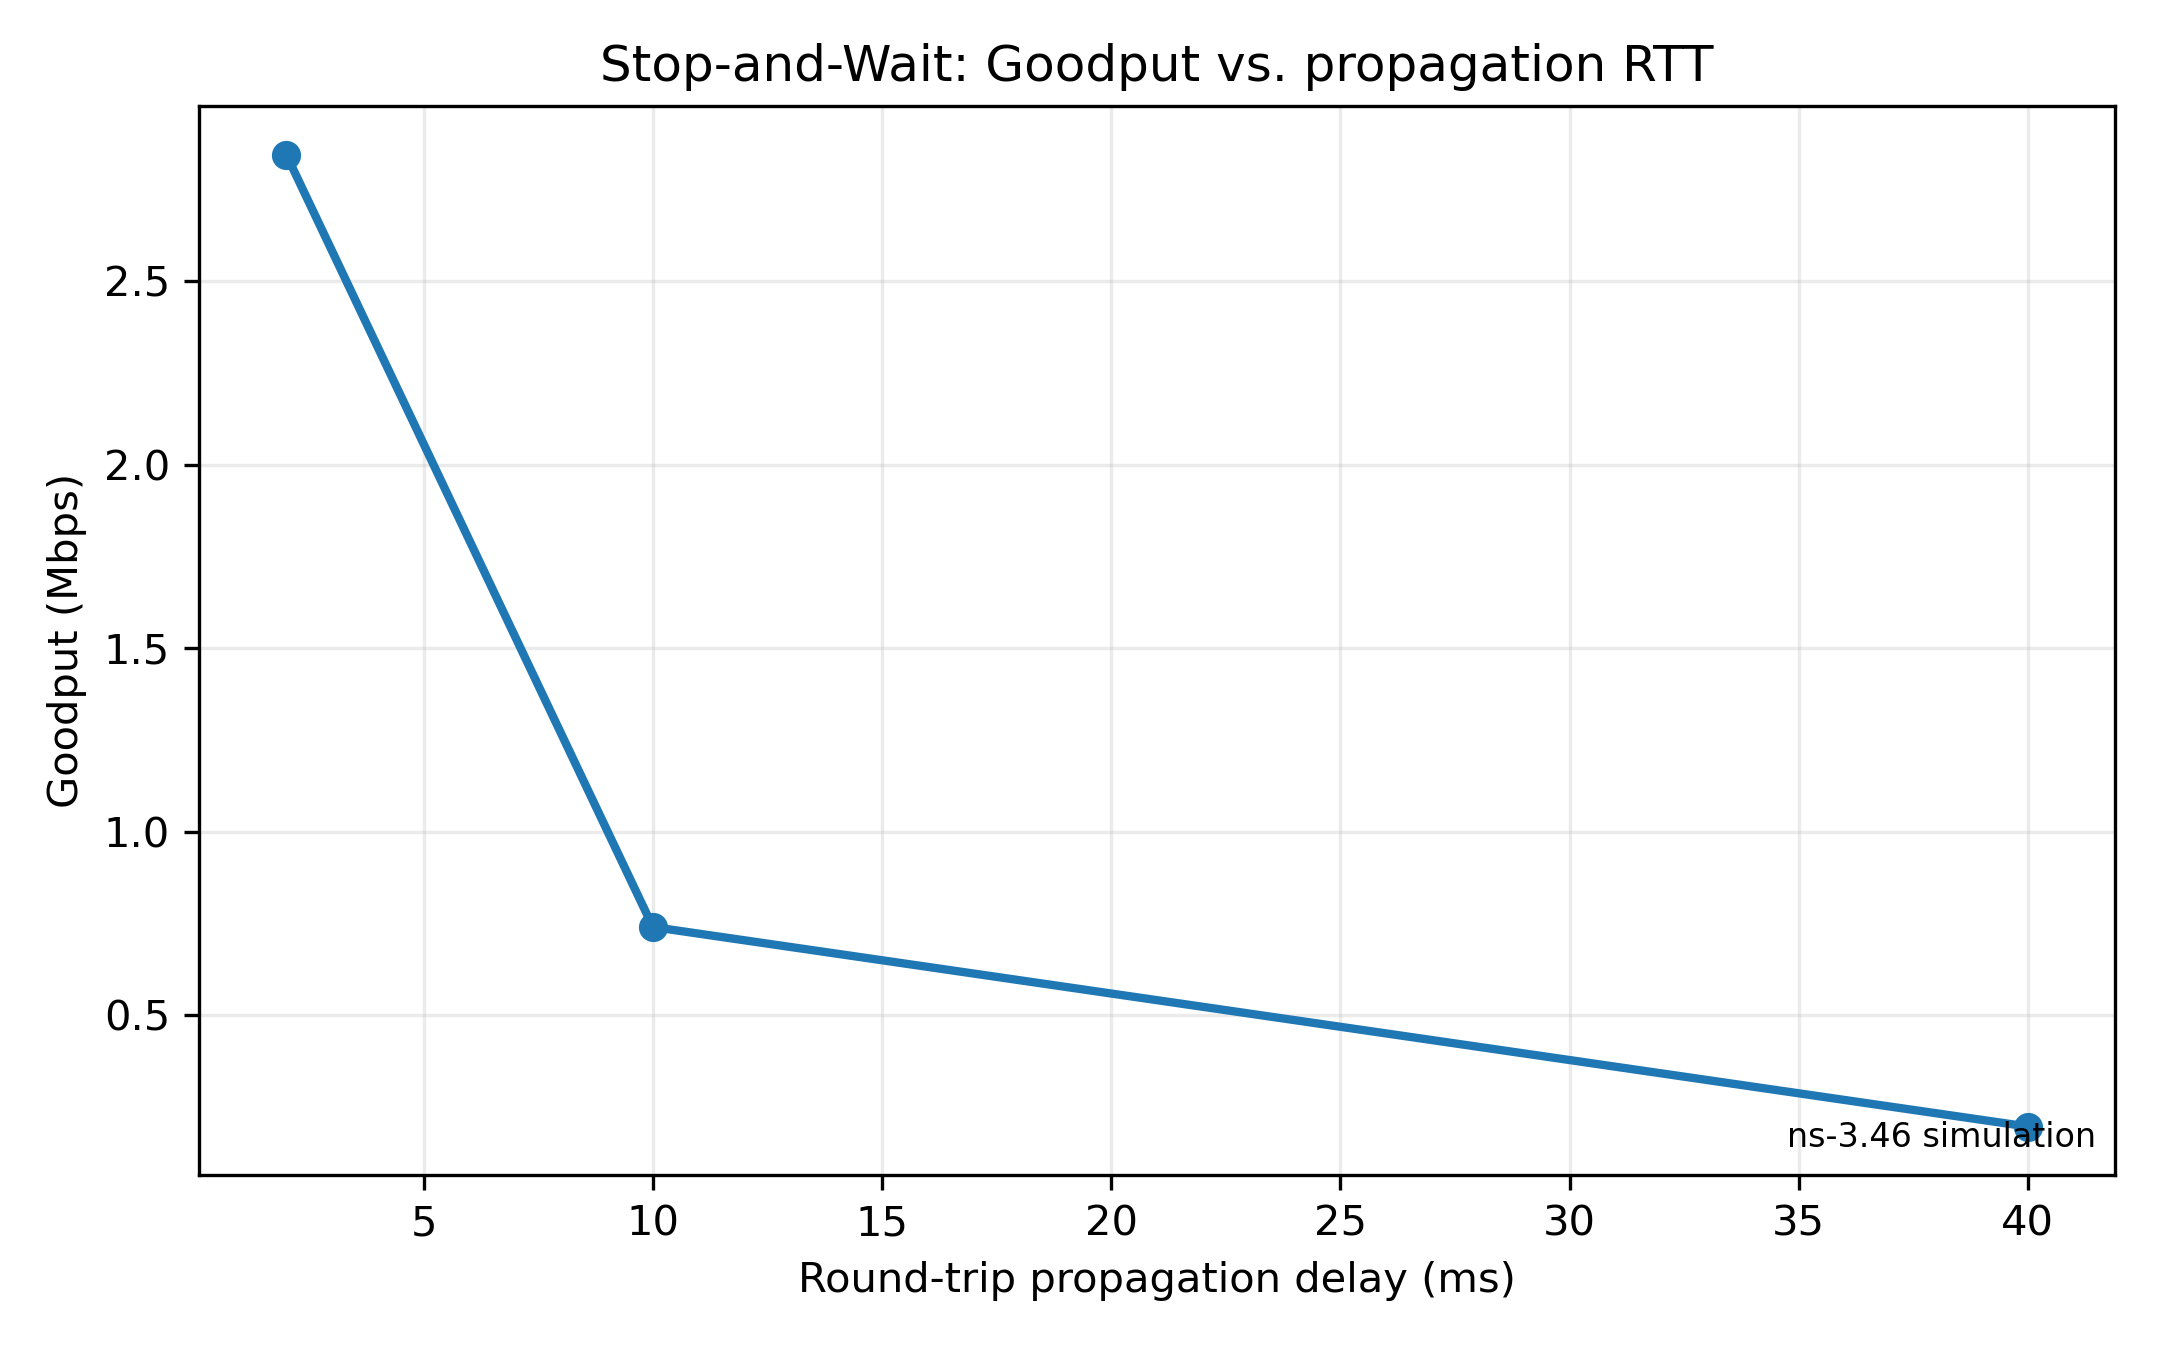
\includegraphics[width=0.82\textwidth]{p1a_stop_wait_delay.png}
\caption{توان‌گذردهی توقف‌و‌انتظار برحسب تأخیر انتشار رفت‌وبرگشت}
\label{fig:sw-delay}
\end{figure}

\begin{table}[H]
\centering
\caption{نتایج توقف‌و‌انتظار در حالت بدون اتلاف}
\begin{tabular}{rrrrr}
\toprule
تأخیر یک‌طرفه (ms) & \en{RTT} انتشار (ms) & توان‌گذردهی (Mbps) & تأخیر متوسط (ms) & بازفرست / انقضا \\
\midrule
\en{1} & \en{2} & \en{2.8456} & \en{1.8056} & \en{0 / 0} \\
\en{5} & \en{10} & \en{0.7400} & \en{5.8056} & \en{0 / 0} \\
\en{20} & \en{40} & \en{0.1960} & \en{20.8056} & \en{0 / 0} \\
\bottomrule
\end{tabular}
\end{table}

برای محمولهٔ \en{1000 byte} روی لینک \en{10 Mbps}، زمان ارسال محموله تقریباً \en{$T_f=0.8 ms$} است. با صرف‌نظر از زمان ارسال \en{ACK} و سربار قاب، تقریب خواسته‌شده در صورت تمرین برابر است با:
\[
U\approx\frac{T_f}{T_f+RTT}.
\]
برای \en{RTT=10 ms} مقدار تقریبی \en{7.41\%} به دست می‌آید. توان‌گذردهی اندازه‌گیری‌شدهٔ \en{0.740 Mbps} نیز تقریباً \en{7.40\%} ظرفیت لینک است و با تقریب سازگار است. با بزرگ شدن تأخیر انتشار، فرستنده مدت بیشتری منتظر تأیید می‌ماند و لینک در فاصلهٔ انتظار بیکار است.

\subsection{اثر اتلاف قاب}
در تأخیر یک‌طرفهٔ پایهٔ \en{5 ms}، احتمال اتلاف مستقل قاب‌های داده و تأیید دریافت برابر \en{0}، ‏\en{0.01}، ‏\en{0.05}، ‏\en{0.10} و ‏\en{0.20} قرار داده شده است.

\begin{figure}[H]
\centering
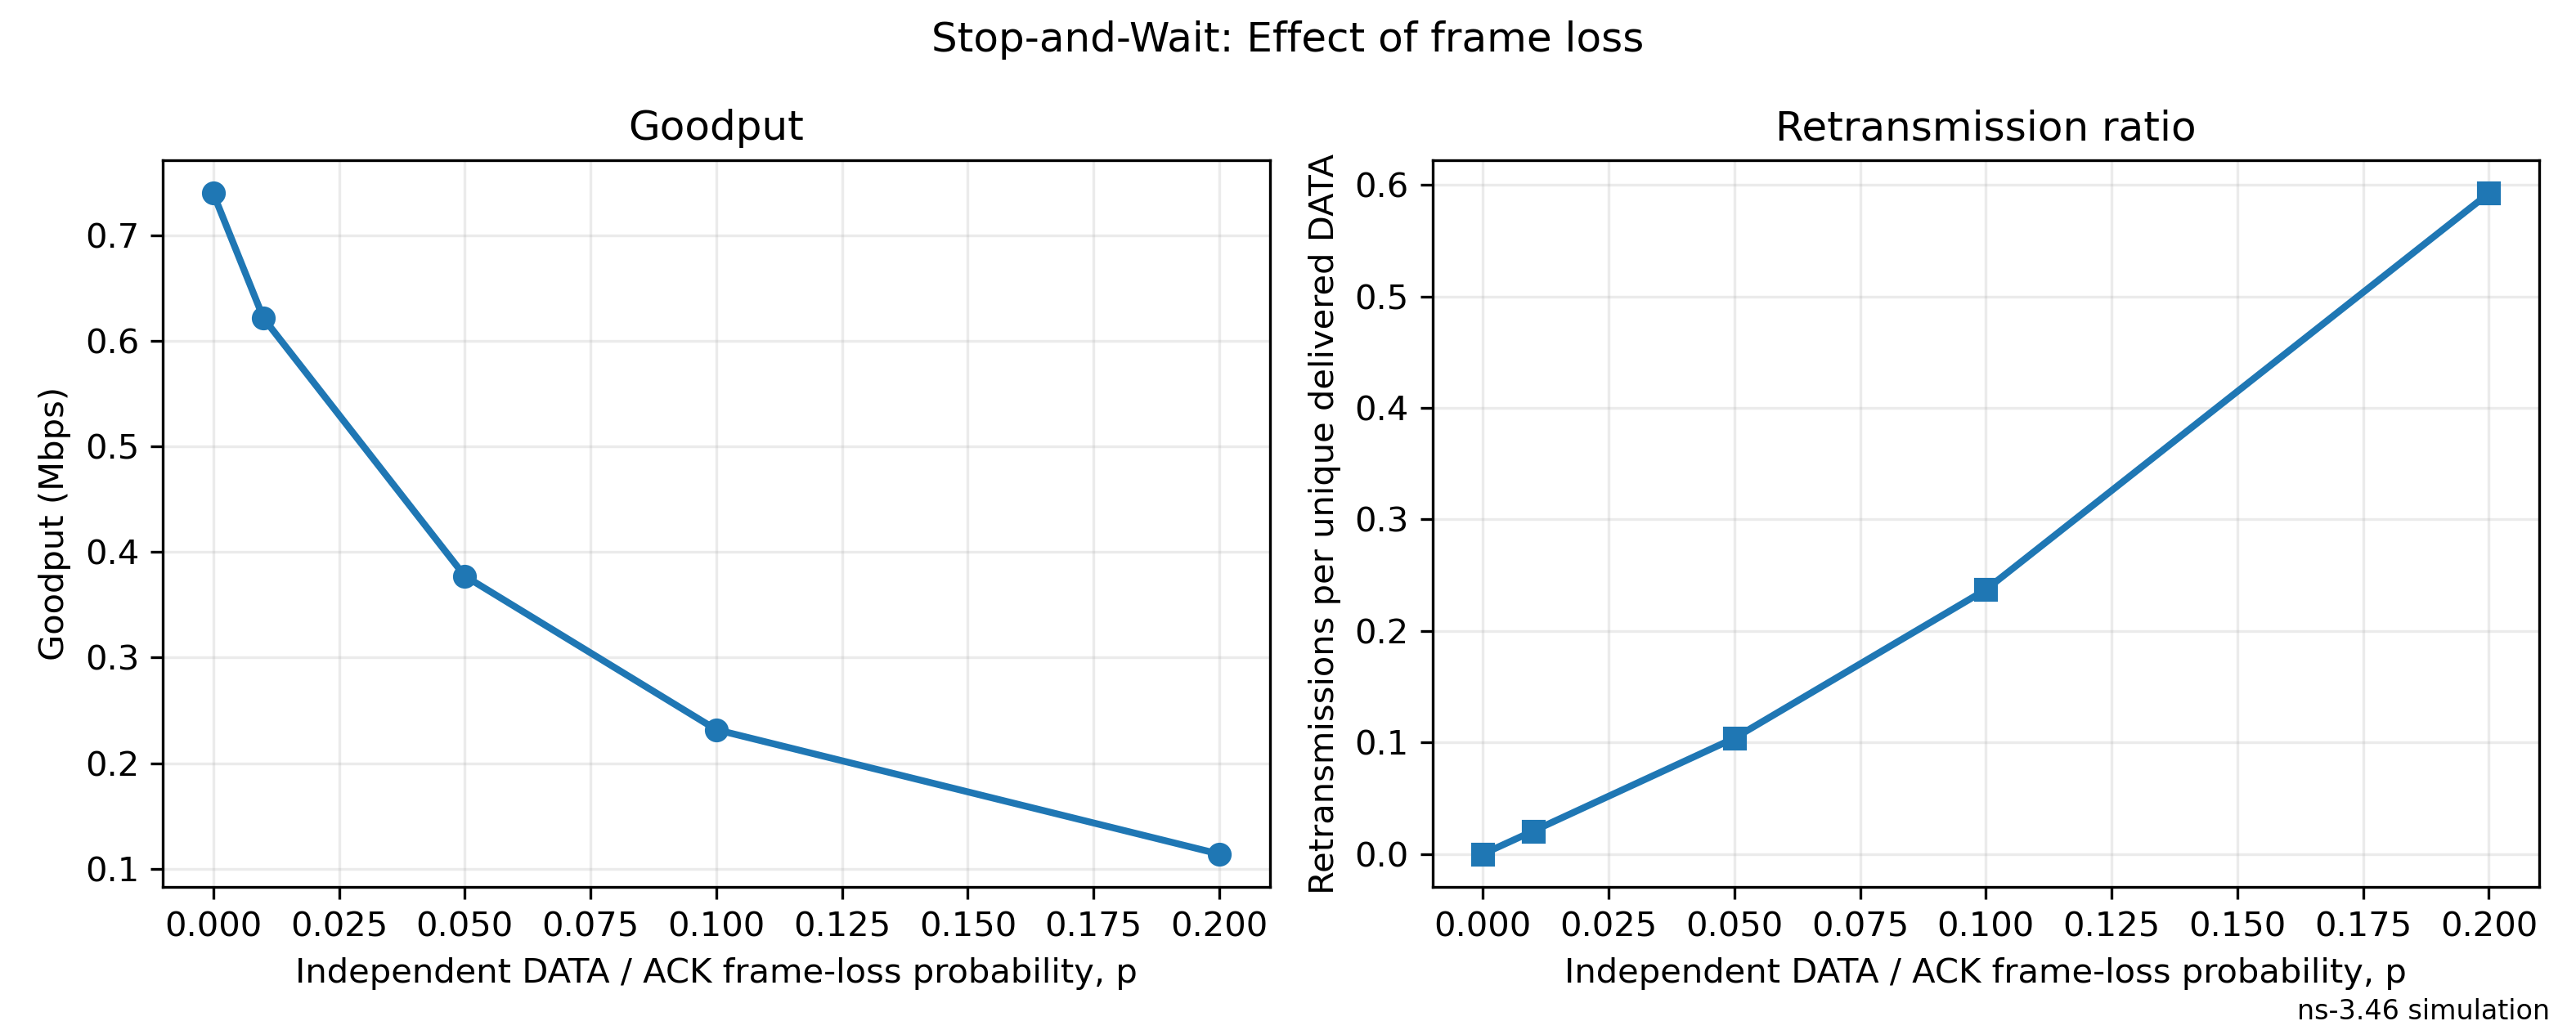
\includegraphics[width=\textwidth]{p1b_stop_wait_loss.png}
\caption{اثر احتمال اتلاف بر توان‌گذردهی و نسبت بازفرست توقف‌و‌انتظار}
\label{fig:sw-loss}
\end{figure}

\begin{table}[H]
\centering
\caption{نتایج توقف‌و‌انتظار در حضور اتلاف}
\begin{tabular}{rrrrrr}
\toprule
\en{$p$} & توان‌گذردهی (Mbps) & نسبت بازفرست & تعداد انقضای زمان‌سنج & اتلاف \en{DATA} & اتلاف \en{ACK} \\
\midrule
\en{0.00} & \en{0.740} & \en{0.000} & \en{0} & \en{0} & \en{0} \\
\en{0.01} & \en{0.614} & \en{0.022} & \en{51} & \en{24} & \en{27} \\
\en{0.05} & \en{0.350} & \en{0.120} & \en{158} & \en{83} & \en{75} \\
\en{0.10} & \en{0.222} & \en{0.252} & \en{210} & \en{115} & \en{95} \\
\en{0.20} & \en{0.116} & \en{0.579} & \en{252} & \en{136} & \en{117} \\
\bottomrule
\end{tabular}
\end{table}

با افزایش \en{$p$}، احتمال موفقیت یک تبادل داده و تأیید آن کاهش می‌یابد. در توقف‌و‌انتظار، گم‌شدن داده یا تأیید باعث انقضای زمان‌سنج و ارسال مجدد همان شمارهٔ توالی می‌شود. گیرنده با شمارهٔ توالی، نسخهٔ تکراری را تشخیص می‌دهد و فقط آن را دوباره تأیید می‌کند؛ تحویل محموله تکرار نمی‌شود. زمان‌سنج بسیار کوتاه می‌تواند پیش از رسیدن تأیید واقعی منقضی شود و بازفرست کاذب ایجاد کند؛ زمان‌سنج بسیار بلند نیز بازیابی پس از اتلاف را کند می‌کند. در این آزمایش زمان‌سنج \en{100 ms} است که از زمان رفت‌وبرگشت پایه به‌مراتب بزرگ‌تر است و به همین دلیل هر اتلاف، وقفهٔ قابل‌توجهی ایجاد می‌کند.

\section{مسئلهٔ دوم: بازگشت به عقب و حاصل‌ضرب پهنای‌باند در تأخیر}
در این بخش، احتمال اتلاف صفر است و اندازهٔ پنجرهٔ فرستنده از مجموعهٔ \en{$W\in\{1,2,4,8,16,32\}$} انتخاب شده است. دو تأخیر یک‌طرفهٔ \en{5 ms} و \en{20 ms} بررسی می‌شوند. گیرنده فقط بستهٔ مورد انتظار را تحویل می‌دهد و بسته‌های خارج از ترتیب را کنار می‌گذارد؛ تأیید تجمعی مقدار شمارهٔ توالی مورد انتظار بعدی را حمل می‌کند.

\begin{figure}[H]
\centering
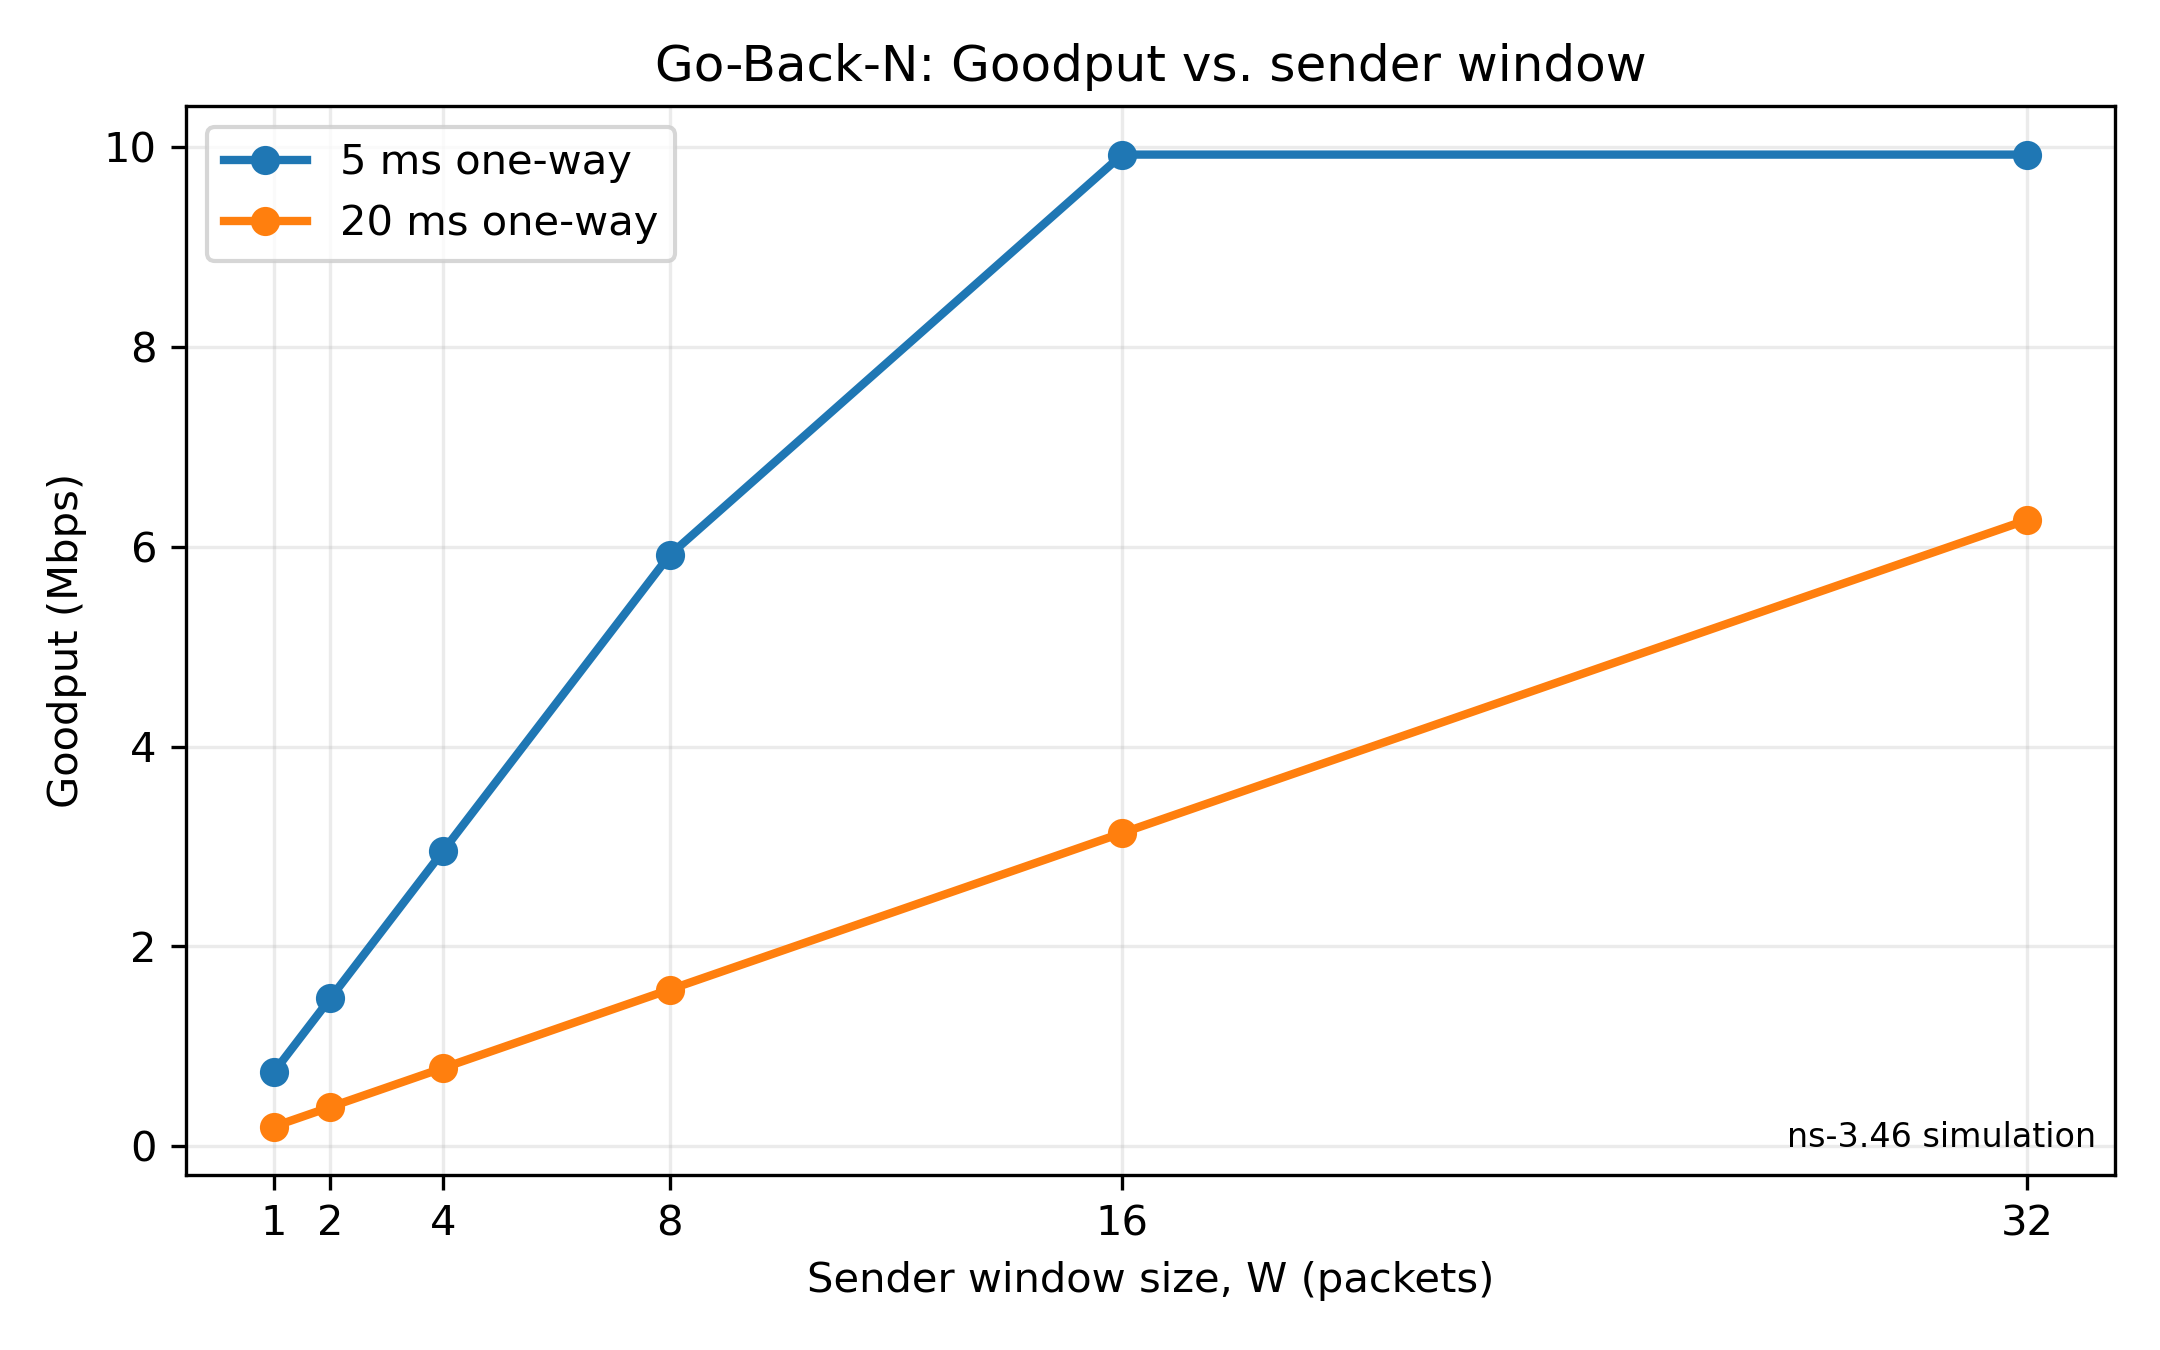
\includegraphics[width=0.82\textwidth]{p2a_gbn_window_goodput.png}
\caption{توان‌گذردهی \en{Go-Back-N} برحسب اندازهٔ پنجره}
\label{fig:gbn-window}
\end{figure}

\begin{table}[H]
\centering
\caption{توان‌گذردهی و تأخیر متوسط \en{Go-Back-N} در دو تأخیر انتشار}
\resizebox{\textwidth}{!}{%
\begin{tabular}{rrrrr}
\toprule
\en{$W$} & توان‌گذردهی در \en{5 ms} (Mbps) & تأخیر متوسط در \en{5 ms} (ms) & توان‌گذردهی در \en{20 ms} (Mbps) & تأخیر متوسط در \en{20 ms} (ms) \\
\midrule
\en{1} & \en{0.740} & \en{5.806} & \en{0.196} & \en{20.806} \\
\en{2} & \en{1.480} & \en{5.806} & \en{0.392} & \en{20.806} \\
\en{4} & \en{2.960} & \en{5.806} & \en{0.784} & \en{20.807} \\
\en{8} & \en{5.919} & \en{5.807} & \en{1.568} & \en{20.809} \\
\en{16} & \en{9.929} & \en{7.886} & \en{3.136} & \en{20.814} \\
\en{32} & \en{9.929} & \en{20.771} & \en{6.271} & \en{20.823} \\
\bottomrule
\end{tabular}}
\end{table}

برای محاسبهٔ \en{BDP} از رابطهٔ \en{$BDP=R\times RTT$} استفاده می‌شود. با نرخ \en{10 Mbps} و محمولهٔ \en{1000 byte}:
\[
\begin{aligned}
RTT_{5ms}&=10ms,& BDP&=100{,}000\;bit=12.5\;kB,& W_{est}&=\lceil 12{,}500/1000\rceil=13,\\
RTT_{20ms}&=40ms,& BDP&=400{,}000\;bit=50\;kB,& W_{est}&=\lceil 50{,}000/1000\rceil=50.
\end{aligned}
\]
در تأخیر \en{5 ms}، پنجرهٔ \en{16} به توان‌گذردهی نزدیک ظرفیت لینک می‌رسد و افزایش آن به \en{32} بهبود بیشتری ایجاد نمی‌کند. این رفتار با تخمین \en{13} بسته سازگار است؛ سربار سرآیندها و زمان ارسال قاب‌ها باعث می‌شود نقطهٔ اشباع دقیقاً با تخمین ساده یکسان نباشد. در تأخیر \en{20 ms}، حتی پنجرهٔ \en{32} نیز از تخمین \en{50} کوچک‌تر است و توان‌گذردهی در حدود \en{6.27 Mbps} باقی می‌ماند.

افزایش پنجره در ابتدا تعداد بسته‌های در حال پرواز را بیشتر می‌کند و زمان انتظار برای تأیید را می‌پوشاند. پس از پر شدن خط، ظرفیت فیزیکی لینک سقف توان‌گذردهی است و بزرگ‌تر کردن پنجره فقط صف و تأخیر را افزایش می‌دهد. پنجرهٔ گیرنده نمونه‌ای از کنترل جریان است؛ این سازوکار سرعت فرستنده را با ظرفیت پذیرش گیرنده هماهنگ می‌کند. کنترل ازدحام شبکه مسئله‌ای متفاوت است و نرخ ارسال را با وضعیت ازدحام مسیر و صف‌های شبکه تنظیم می‌کند. در این آزمایش یک مسیر نقطه‌به‌نقطه و بدون سازوکار کنترل ازدحام شبکه وجود دارد.

\section{مسئلهٔ سوم: تکرار انتخابی و بافر گیرنده}
\subsection{مقایسهٔ \en{Go-Back-N} و \en{Selective Repeat}}
در این مقایسه، شرایط پایه یکسان است: تأخیر یک‌طرفهٔ \en{5 ms}، احتمال اتلاف مستقل \en{0.05} برای داده و تأیید، زمان‌سنج \en{100 ms}، محمولهٔ \en{1000 byte} و بافر گیرندهٔ \en{20} بسته. اندازهٔ پنجره در هر دو پروتکل از مجموعهٔ خواسته‌شده انتخاب می‌شود.

\begin{figure}[H]
\centering
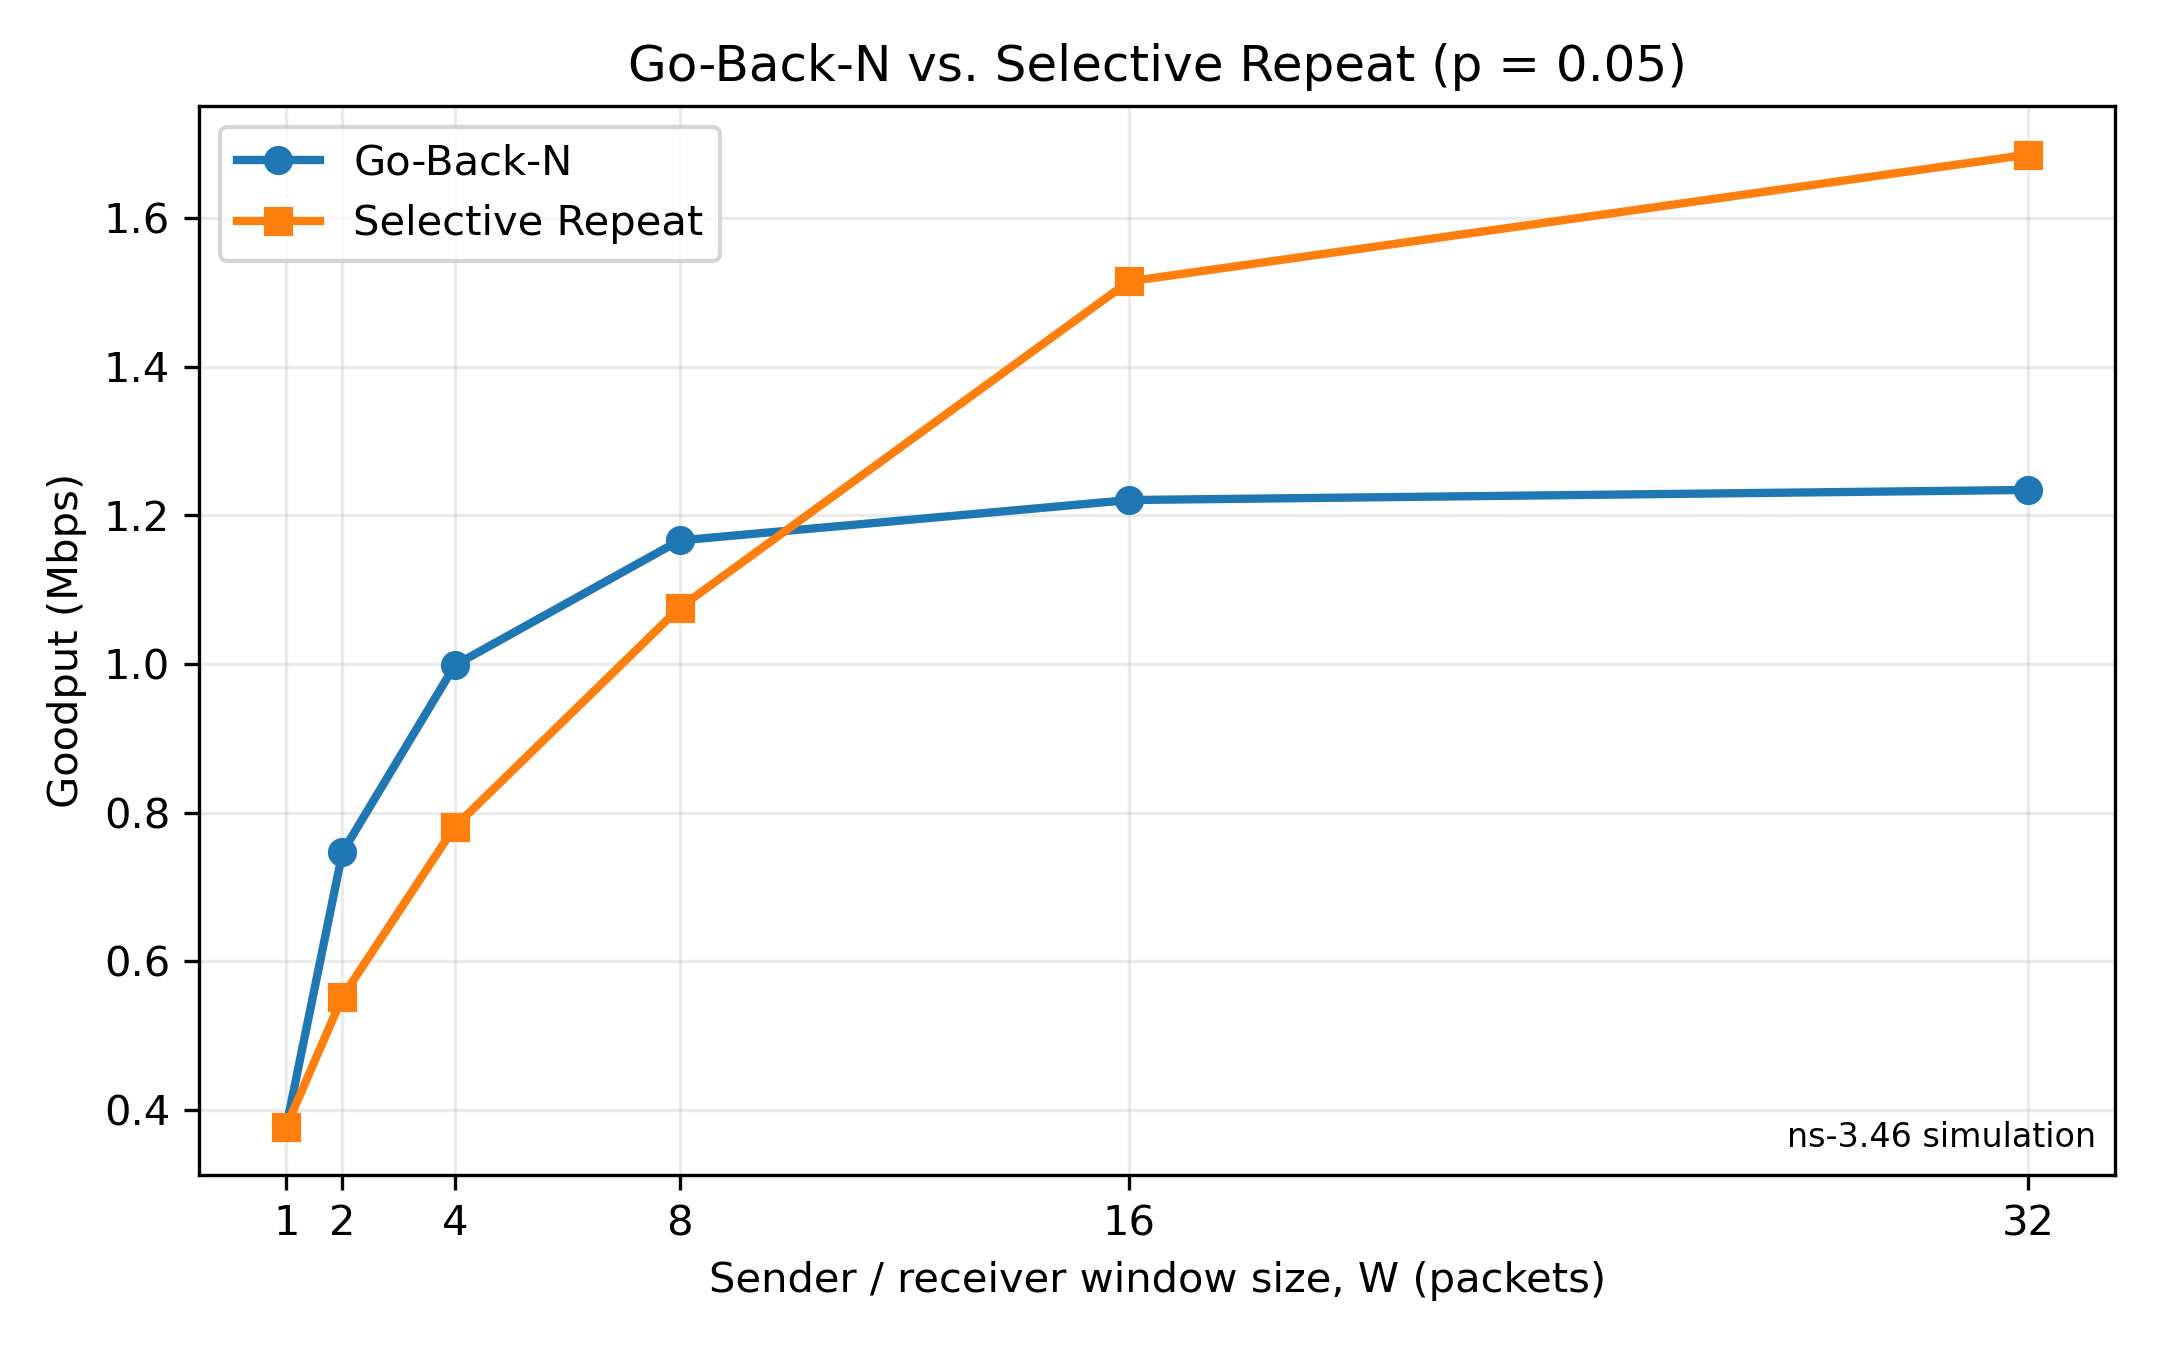
\includegraphics[width=0.82\textwidth]{p3a_gbn_vs_sr_goodput.png}
\caption{مقایسهٔ توان‌گذردهی دو پروتکل در احتمال اتلاف \en{0.05}}
\label{fig:gbn-sr}
\end{figure}

\begin{table}[H]
\centering
\small
\caption{مقایسهٔ توان‌گذردهی، تأخیر و بازفرست در \en{Go-Back-N} و \en{Selective Repeat}}
\begin{tabular}{crrrr}
\toprule
پروتکل & \en{$W$} & توان‌گذردهی (Mbps) & تأخیر متوسط (ms) & بازفرست به‌ازای هر بسته \\
\midrule
\en{GBN} & \en{1} & \en{0.350} & \en{11.594} & \en{0.120} \\
\en{GBN} & \en{2} & \en{0.654} & \en{18.704} & \en{0.131} \\
\en{GBN} & \en{4} & \en{0.929} & \en{29.207} & \en{0.222} \\
\en{GBN} & \en{8} & \en{1.127} & \en{51.496} & \en{0.426} \\
\en{GBN} & \en{16} & \en{1.163} & \en{104.971} & \en{0.888} \\
\en{GBN} & \en{32} & \en{1.147} & \en{216.152} & \en{1.793} \\
\midrule
\en{SR} & \en{1} & \en{0.350} & \en{11.594} & \en{0.120} \\
\en{SR} & \en{2} & \en{0.497} & \en{17.391} & \en{0.117} \\
\en{SR} & \en{4} & \en{0.693} & \en{25.374} & \en{0.115} \\
\en{SR} & \en{8} & \en{1.035} & \en{34.777} & \en{0.105} \\
\en{SR} & \en{16} & \en{1.460} & \en{53.523} & \en{0.106} \\
\en{SR} & \en{32} & \en{1.579} & \en{126.673} & \en{0.467} \\
\bottomrule
\end{tabular}
\end{table}

در \en{Go-Back-N}، اگر بسته‌ای از دست برود، گیرنده بسته‌های بعدی خارج از ترتیب را دور می‌اندازد و تأیید تجمعی شمارهٔ مورد انتظار را اعلام می‌کند. پس از پایان زمان‌سنج، فرستنده همهٔ بسته‌های معلق از قدیمی‌ترین بسته به بعد را دوباره می‌فرستد. در \en{Selective Repeat} هر بسته تأیید مستقل دارد و گیرنده می‌تواند بسته‌های خارج از ترتیب را موقتاً ذخیره کند؛ در نتیجه فقط بستهٔ گم‌شده یا تأییدنشده دوباره ارسال می‌شود.

در داده‌های این اجرای مرجع، برای پنجرهٔ \en{32} توان‌گذردهی \en{SR} حدود \en{1.579 Mbps} و برای \en{GBN} حدود \en{1.147 Mbps} است. همچنین نسبت بازفرست در \en{SR} کمتر است. در پنجره‌های کوچک‌تر، برتری \en{SR} در این نمونهٔ تصادفی یکنواخت نیست؛ از دست رفتن \en{ACK} و زمان‌سنج نسبتاً بلند می‌تواند باعث شود تأیید تجمعی \en{GBN} چند بسته را یک‌جا تأیید کند، در حالی که \en{SR} برای بسته‌ای با تأیید ازدست‌رفته منتظر بازفرست جداگانه می‌ماند. بنابراین نتیجه به الگوی تصادفی اتلاف و اندازهٔ پنجره نیز وابسته است.

\subsection{اثر ظرفیت بافر گیرنده در \en{Selective Repeat}}
برای این آزمایش \en{$W=32$} ثابت است و ظرفیت بافر خارج از ترتیب از مجموعهٔ \en{$B_{rx}\in\{4,8,16,32,64\}$} انتخاب می‌شود. سیاست سرریز این است که اگر بافر پر باشد، بستهٔ خارج از ترتیب بدون ارسال \en{ACK} حذف می‌شود؛ فرستنده پس از انقضای زمان‌سنج همان بسته را مجدداً می‌فرستد. بستهٔ مورد انتظار در صورت رسیدن، مستقیماً تحویل می‌شود و ظرفیت بافر را اشغال نمی‌کند.

\begin{figure}[H]
\centering
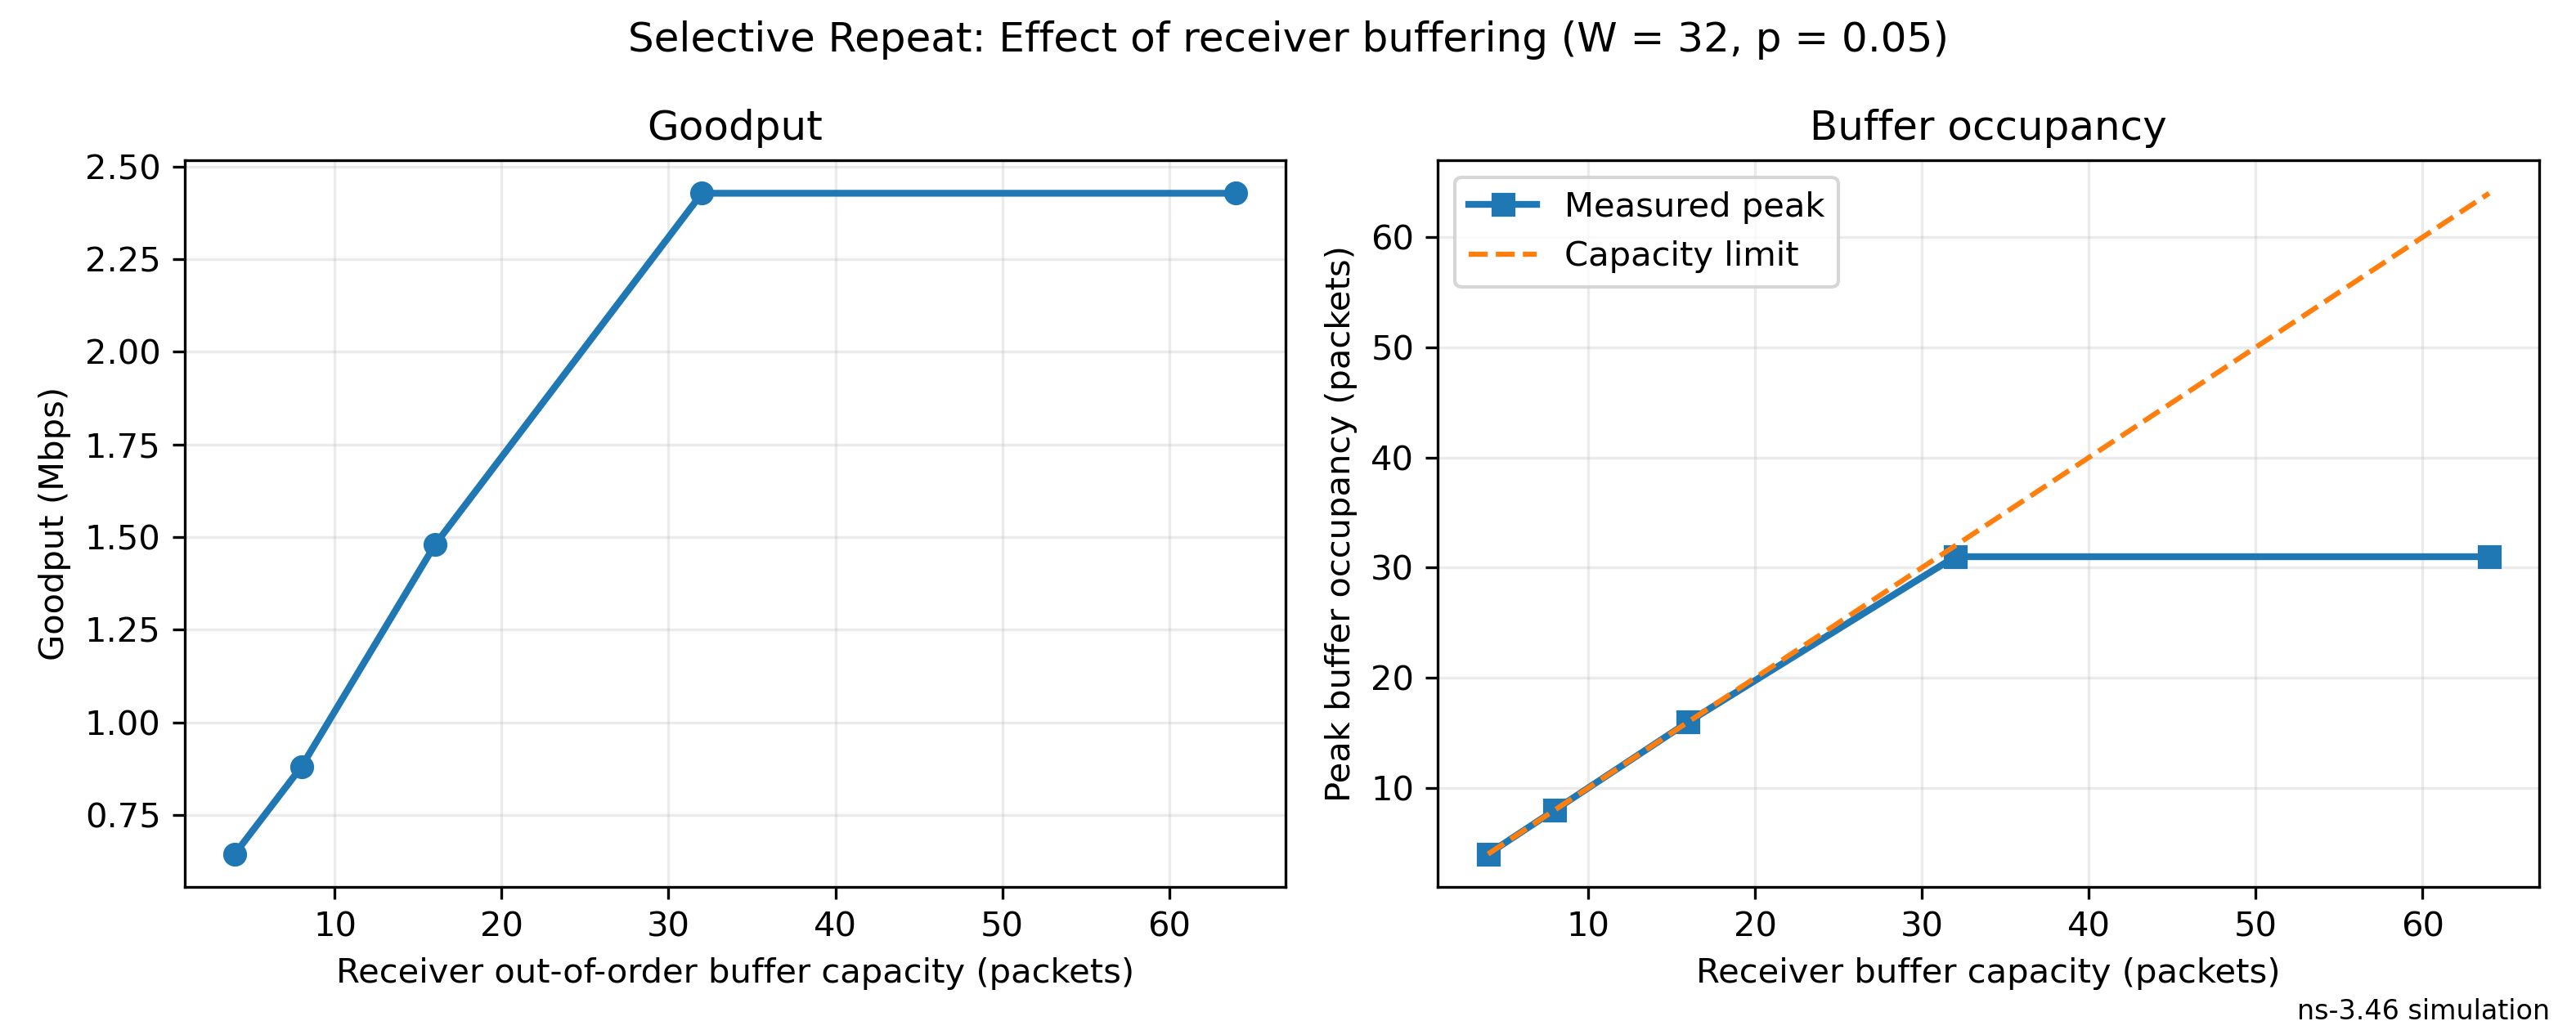
\includegraphics[width=\textwidth]{p3b_sr_buffer_capacity.png}
\caption{اثر ظرفیت بافر بر توان‌گذردهی و بیشینهٔ اشغال بافر در \en{Selective Repeat}}
\label{fig:sr-buffer}
\end{figure}

\begin{table}[H]
\centering
\caption{نتایج ظرفیت بافر و کنترل سرریز}
\begin{tabular}{rrrrr}
\toprule
ظرفیت بافر (بسته) & توان‌گذردهی (Mbps) & بیشینهٔ اشغال (بسته) & سرریز & رعایت حد ظرفیت \\
\midrule
\en{4} & \en{0.565} & \en{4} & \en{7053} & بله \\
\en{8} & \en{0.729} & \en{8} & \en{5867} & بله \\
\en{16} & \en{1.283} & \en{16} & \en{3186} & بله \\
\en{32} & \en{2.276} & \en{31} & \en{0} & بله \\
\en{64} & \en{2.276} & \en{31} & \en{0} & بله \\
\bottomrule
\end{tabular}
\end{table}

با افزایش ظرفیت از \en{4} به \en{32} بسته، تعداد سرریزها کاهش و توان‌گذردهی افزایش می‌یابد. برای پنجرهٔ \en{32} حداکثر \en{31} بسته می‌توانند خارج از ترتیب و پشت یک بستهٔ مفقود قرار بگیرند؛ بنابراین ظرفیت \en{64} نسبت به \en{32} سود اضافه‌ای ایجاد نمی‌کند. ستون بیشینهٔ اشغال نشان می‌دهد در تمام آزمایش‌ها مقدار بافر از ظرفیت تعیین‌شده فراتر نرفته است.

\section{بحث و جمع‌بندی}
\begin{itemize}
  \item توقف‌و‌انتظار ساده است و با شمارهٔ توالی و بازتأیید نسخه‌های تکراری، تحویل یکتا را تضمین می‌کند؛ اما با افزایش \en{RTT} بهره‌وری آن به‌شدت کاهش می‌یابد.
  \item پنجرهٔ لغزان در \en{Go-Back-N} امکان ارسال چند بسته بدون انتظار برای تأیید هر بسته را می‌دهد. اندازهٔ پنجرهٔ لازم با \en{BDP} افزایش می‌یابد و پس از اشباع لینک، افزایش بیشتر پنجره فقط تأخیر صف را بیشتر می‌کند.
  \item \en{Selective Repeat} با تأیید مستقل و بازفرست انتخابی از بازفرست غیرضروری بسته‌های سالم جلوگیری می‌کند، اما به بافر خارج از ترتیب و مدیریت زمان‌سنج جداگانه نیاز دارد.
  \item بافر محدود در \en{Selective Repeat} می‌تواند باعث حذف بسته‌های خارج از ترتیب و تأخیر در بازیابی شود. سیاست حذف بدون تأیید باعث می‌شود فرستنده پس از زمان‌سنج مجدداً تلاش کند و اشغال بافر هرگز از ظرفیت تعریف‌شده بیشتر نشود.
  \item پنجرهٔ گیرنده و ظرفیت بافر، ابزار کنترل جریان‌اند؛ این پروژه کنترل ازدحام شبکه را پیاده‌سازی نمی‌کند.
\end{itemize}

\section{تکرارپذیری و محدودیت نسخهٔ تحویلی}
کد اصلی در \en{scratch/arq-hw3.cc} همهٔ سناریوهای موردنیاز را با \en{--mode=all} اجرا می‌کند و خروجی خام را در قالب \en{CSV} می‌نویسد. فایل \en{README.txt} دستورات دقیق اجرای تصویر Docker درس، اجرای شبیه‌سازی، تولید نمودار و کامپایل گزارش را ارائه می‌کند. پارامترهای نرخ لینک، تأخیر، اندازهٔ محموله، زمان شبیه‌سازی، زمان‌سنج، احتمال اتلاف، پنجره، ظرفیت بافر و بذر تصادفی از خط فرمان قابل تغییرند.

\textbf{یادآوری نهایی:} اعداد و نمودارهای این فایل برچسب «مدل مرجع رویدادگسسته» دارند. پیش از تحویل دانشگاهی، برنامهٔ \en{ns-3} را طبق \en{README.txt} در محیط Docker اجرا کنید، خروجی \en{results/ns3\_results.csv} را تولید کنید، نمودارها را از همان فایل بسازید و گزارش را دوباره با \en{XeLaTeX} کامپایل کنید. تا پیش از این مرحله، نباید داده‌های پیش‌نمایش به‌عنوان اندازه‌گیری مستقیم \en{ns-3} گزارش شوند.

\end{document}
